\documentclass[10pt]{memoir}
\setstocksize{220mm}{155mm} 	        
\settrimmedsize{220mm}{155mm}{*}	
\settypeblocksize{170mm}{116mm}{*}	
\setlrmargins{18mm}{*}{*}
\setulmargins{*}{*}{1.2}
%\setlength{\headheight}{5pt}%
\checkandfixthelayout[lines]
\linespread{1.16}
\flushbottom

%%% Hyphenation settings
\usepackage[htt]{hyphenat}
\hyphenation{he-lio-trope opos-sum}
\tracingparagraphs=1
%Hyphenation in Devanāgarī of the edition still missing? Probably this needs to be modified in babel-iast package? 

%%% babel
\usepackage[english]{babel}
\usepackage{babel-iast/babel-iast}

\babelfont[iast]{rm}[Renderer=Harfbuzz, Scale=1.3]{AdishilaSan}%AdishilaSan}
\babelfont[english]{rm}{Adobe Text Pro}

%%% more functionality
\PassOptionsToPackage{hyphens}{url}
\usepackage{hyperref}
\usepackage{pdflscape}
\usepackage{cleveref}
\usepackage{url}
\usepackage{cleveref}
\usepackage{microtype}
\usepackage{lineno}

%\usepackage{bigfoot}
%%% more functions
\usepackage[dvipsnames]{xcolor}
%\usepackage[para,perpage]{footmisc}

%%%für den Counter von Kapiteln und Sätzen! 
\newcommand{\uproman}[1]{\uppercase\expandafter{\romannumeral#1}}
\newcommand{\lowroman}[1]{\romannumeral#1\relax}

\makeindex
\newfontfamily\sanskritfont[Script=Devanagari,Mapping=RomDev,Scale=1.1]{Sanskrit2003}
\usepackage{pifont,fourier-orns,lettrine,psvectorian,paralist,enumitem,pdfpages,wrapfig,tabulary,lettrine,longtable}
\setlist[enumerate]{itemsep=0mm}
\usepackage[autostyle]{csquotes}
\usepackage[defaultlines=2,all]{nowidow}
\usepackage{ellipsis,adforn,booktabs,longtable,url,tikz}
\lineskiplimit=-3pt          

\makechapterstyle{IeT}{%
  \chapterstyle{default}
  \renewcommand*{\printchapternonum}{\centering}
  \renewcommand*{\clearforchapter}{\cleartorecto} 
  \aliaspagestyle{chapter}{empty}}
\chapterstyle{IeT}
\setsecnumdepth{none}  \openright  \nouppercaseheads
\settocdepth{subsubsection}

%%%% test better pagebreaks
%\def\fussy{%
%  \emergencystretch\z@
%  \tolerance 200%
%  \hfuzz .1\p@
%  \vfuzz\hfuzz}

%\interfootnotelinepenalty=10000\relax

%\usepackage[maxfloats=256]{morefloats}

%\maxdeadcycles=500

%raggedbottomsectiontrue
%%\checkandfixthelayout


%%%%%%%  biblatex
%\newcommand{\noun}[1]{\textsc{#1}}    %  philosophy-verbose
\usepackage[backend=biber, sorting=nyt, style=verbose]{biblatex} %%%%ORIGINAL TiE
\renewcommand*{\mkbibnamefamily}[1]{\textsc{#1}}


\DeclareFieldFormat{url}{%
  \mkbibacro{URL}\addcolon\space
  \href{#1}{\nolinkurl{\thefield{urlraw}}}}

\DeclareFieldFormat{citeurl}{%
  \href{#1}{\nolinkurl{\thefield{urlraw}}}} 


\DeclareFieldFormat{postnote}{#1}
\renewcommand{\postnotedelim}{, }
\addbibresource{bindu.bib}

%%% ekdosis
\usepackage[teiexport=tidy,parnotes=true]{ekdosis}% =tidy cleans up HTML and XML documents by fixing markup errors and upgrading legacy code to modern standards. parnotes=footnotes below or above critical apparatus

\SetLineation{lineation=page, modulo} %lineation=page sets thenumbering to start afresh at the top of each page. =modulo makes every fifth line numbered. {lineation=page} makes every line numbered! 

\renewcommand{\linenumberfont}{\selectlanguage{english}\footnotesize} %sets language of lines to English

\SetTEIxmlExport{autopar=false} %autopar=falseinstructs ekdosis to ignore blank lines in the.tex sourcefile as markers for paragraph boundaries. As a result, each paragraph of the edition must be found within an environment associated with the xml <p> element

\SetHooks{
  lemmastyle=\bfseries,
  %refnumstyle=\selectlanguage{english}\bfseries,
  refnumstyle=\selectlanguage{english}\color{blue}\bfseries,
  appheight=0.8\textheight,
}

\newif\ifinapparatus
\DeclareApparatus{source}[
%bhook=\inapparatustrue,
lang=english,
notelang=english,
% bhook=\selectlanguage{english},
bhook=\selectlanguage{english}\textbf{Sources:},%
%maxentries=4, 
%ehook=.]
%sep={] },
%nosep,
]

\newif\ifinapparatus
\DeclareApparatus{testium}[
%bhook=\inapparatustrue,
lang=english,
notelang=english,
% bhook=\selectlanguage{english},
bhook=\selectlanguage{english}\textbf{Testimonia:},
%maxentries=4, 
%ehook=.]
%nosep, 
]

% Declare \ifinapparatus and set \inapparatustrue at the beginning of
% the apparatus criticus block. Also set the language.  
\newif\ifinapparatus
  \DeclareApparatus{default}[
  %bhook=\inapparatustrue, 
  lang=english,
  %maxentries=33,
  %bhook=\selectlanguage{english},
  sep = {] },
  delim=\hskip 0.75em,
  rule=\rule{0.7in}{0.4pt},
]

\newif\ifinapparatus
\DeclareApparatus{philcomm}[
%bhook=\inapparatustrue,
lang=english,
notelang=english,
bhook=\selectlanguage{english}\textbf{Philological Commentary:},
%bhook=\selectlanguage{english},
sep={: },
]

\ekdsetup{
showpagebreaks,
spbmk = \textcolor{blue}{spb},
hpbmk = \textcolor{red}{hpb}
}

%\usepackage{fnpos}
%\makeFNmid
%\makeFNbottom
\usepackage[bottom]{footmisc}
%%%%%%%%%%%%%%%%%%%%%%%%%%%
\makeatletter
\def\blfootnote{\gdef\@thefnmark{}\@footnotetext}
\makeatother
%%%%%%%%%%%%%%%%%%%%%%%%%


% Macros and Definitions for the Print of Sigla
\def\acpc#1#2#3{{#1}\rlap{\textrm{\textsuperscript{#3}}}\textsubscript{\textrm{#2}}\space}
\def\sigl#1#2{{{#1}}\textsubscript{\textrm{#2}}}
\def\None{{\sigl{N}{1}}} \def\Noneac{\acpc{N}{1}{ac}\,} \def\Nonepc{\acpc{N}{1}{pc}\,}
\def\Ntwo{{\sigl{N}{2}}} \def\Noneac{\acpc{N}{2}{ac}\,} \def\Nonepc{\acpc{N}{2}{pc}\,}
\def\Done{{\sigl{D}{1}}} \def\Doneac{\acpc{D}{1}{ac}\,} \def\Donepc{\acpc{D}{1}{pc}\,}
\def\Dtwo{{\sigl{D}{2}}} \def\Dtwoac{\acpc{D}{2}{ac}\,} \def\Dtwopc{\acpc{D}{2}{pc}\,}
\def\Uone{{\sigl{U}{1}}} \def\Uoneac{\acpc{U}{1}{ac}\,} \def\Uonepc{\acpc{U}{1}{pc}\,}                 
\def\Utwo{{\sigl{U}{2}}} \def\Utwoac{\acpc{U}{2}{ac}\,} \def\Utwopc{\acpc{U}{2}{pc}\,}

%%%%%%%%%%%%%% Tattvabinduyoga - List of Witnesses   %%%%%%%%%%%%%%%%%%%
\DeclareWitness{ceteri}{\selectlanguage{english}cett.}{ceteri}[]   
\DeclareWitness{E}{\selectlanguage{english}E}{Printed Edition}[]    
\DeclareWitness{P}{\selectlanguage{english}P}{Pune BORI 664}[]  
\DeclareWitness{B}{\selectlanguage{english}B}{Bodleian 485}[]       
\DeclareWitness{N1}{\selectlanguage{english}N\textsubscript{1}}{NGMPP 38/31}[]
\DeclareWitness{N2}{\selectlanguage{english}N\textsubscript{2}}{NGMPP B 38/35}[]
\DeclareWitness{L}{\selectlanguage{english}L}{LALCHAND 5876}[]  
\DeclareWitness{D}{\selectlanguage{english}D}{IGNCA 30019}[] 
%\DeclareWitness{D2}{\selectlanguage{english}D\textsubscript{2}}{IGNCA 30020}[]  
\DeclareWitness{U1}{\selectlanguage{english}U\textsubscript{1}}{SORI 1574}[] 
\DeclareWitness{U2}{\selectlanguage{english}U\textsubscript{2}}{SORI 6082}[]
%%%%%%%%%%%%%% Tattvabinduyoga - Groups of Witnesses   %%%%%%%%%%%%%%%%%%%
\DeclareWitness{X}{\selectlanguage{english}\alpha}{Alpha Group: D,N1,N2,U1}[]
\DeclareWitness{Y}{\selectlanguage{english}\beta}{Beta Group: B,E,L,P,U2}[]
%%%%%%%%%%%%% Testimonia
\DeclareWitness{Ysv}{\selectlanguage{english}Ysv}{Yogasvarodaya}[] %%%add infos!  

%%%%%%%%%%%%%%%%%%%%%%%%%%%%%%%%%%%%%%%%%%%
% Macro for Editing Abbrevs.
\def\om{\textrm{\footnotesize \textit{om.}\ }} %prints om. for omitted in apparatus
\def\korr{\textrm{\footnotesize \textit{em.}\ }} %prints em. for emended in apparatus
\def\conj{\textrm{\footnotesize \textit{conj.}\ }} %prints conj. for conjectured in apparatus

% \supplied{text} EDITORIAL ADDITION -> Within \lem oder \rdg
% \surplus{text} EDITORIAL DELETION -> Within \lem oder \rdg
% \sic{text} CRUX
% \gap{text} LACUNAE -> [reason=??, unit=??, quantity=??, extent=??]


%%%%%%%%%%%%%%%%%%%%%%%%%%%%%%%%%%%%%%%%%%% All macros of this list can be used in 
% Macro for Editing Abbrevs.
\def\eyeskip{\textrm{{ab.\,oc. }}}
\def\aberratio{\textrm{{ab.\,oc. }}}
\def\ad{\textrm{{ad}}}
\def\add{\textrm{{add.\ }}}
\def\ann{\textrm{{ann.\ }}}
\def\ante{\textrm{{ante }}} 
\def\post{\textrm{{post }}}
%\def\ceteri{cett.\,}                   
\def\codd{\textrm{{codd.\ }}}

\def\coni{\textrm{{coni.\ }}}
\def\contin{\textrm{{contin.\ }}}
\def\corr{\textrm{{corr.\ }}}
\def\del{\textrm{{del.\ }}}
\def\dub{\textrm{{ dub.\ }}}

\def\expl{\textrm{{explic.\ }}} 
\def\explica t{\textrm{{explic.\ }}}
\def\fol{\textrm{{fol.\ }}}
\def\foll{\textrm{{foll.\ }}}
\def\gloss{\textrm{{glossa ad }}}
\def\ins{\textrm{{ins.\ }}}      
\def\inseruit{\textrm{{ins.\ }}} 
\def\im{{\kern-.7pt\lower-1ex\hbox{\textrm{\tiny{\emph{i.m.}}}\kern0pt}}} %\textrm{\scriptsize{i.m.\ }}}      
\def\inmargine{{\kern-.7pt\lower-.7ex\hbox{\textrm{\tiny{\emph{i.m.}}}\kern0pt}}}%\textrm{\scriptsize{i.m.\ }}}      
\def\intextu{{\kern-.7pt\lower-.95ex\hbox{\textrm{\tiny{\emph{i.t.}}}\kern0pt}}}%\textrm{\scriptsize{i.t.\ }}}           
\def\indist{\textrm{{indis.\ }}}  
\def\indis{\textrm{{indis.\ }}}
\def\iteravit{\textrm{{iter.\ }}} 
\def\iter{\textrm{{iter.\ }}}
\def\lectio{\textrm{{lect.\ }}}   
\def\lec{\textrm{{lect.\ }}}
\def\leginequit{\textrm{{l.n. }}} 
\def\legn{\textrm{{l.n. }}}
\def\illeg{\textrm{{l.n. }}}

\def\primman{\textrm{{pr.m.}}}
\def\prob{\textrm{{prob.}}}
\def\rep{\textrm{{repetitio }}}
\def\secundamanu{\textrm{\scriptsize{s.m.}}}            \def\secm{{\kern-.6pt\lower-.91ex\hbox{\textrm{\tiny{\emph{s.m.}}}\kern0pt}}}%   \textrm{\scriptsize{s.m.}}}
\def\sequentia{\textrm{{seq.\,inv.\ }}}  
\def\seqinv{\textrm{{seq.\,inv.\ }}}
\def\order{\textrm{{seq.\,inv.\ }}}
\def\supralineam{{\kern-.7pt\lower-.91ex\hbox{\textrm{\tiny{\emph{s.l.}}}\kern0pt}}} %\textrm{\scriptsize{s.l.}}}
\def\interlineam{{\kern-.7pt\lower-.91ex\hbox{\textrm{\tiny{\emph{s.l.}}}\kern0pt}}}   %\textrm{\scriptsize{s.l.}}}
\def\vl{\textrm{v.l.}}   \def\varlec{\textrm{v.l.}} \def\varialectio{\textrm{v.l.}}
\def\vide{\textrm{{cf.\ }}}
\def\cf{\textrm{{cf.\ }}} 
\def\videtur{\textrm{{vid.\,ut}}}
\def\crux{\textup{[\ldots]} }
\def\cruxx{\textup{[\ldots]}}
\def\unm{\textit{unm.}}
%%%%%%%%%%%%%%%%%%%%%%%%%%%%%%%%%%%%

% List of Scholars
\DeclareScholar{ego}{ego}[
forename=Nils Jacob,
surname=Liersch]

% Persons:14\DeclareScholar{ego}{ego}[15forename=Robert,16surname=Alessi]17% Useful shorthands:18\DeclareShorthand{codd}{codd.}{V,I,R,H}19\DeclareShorthand{edd}{edd.}{Lit,Erm,Sm}20\DeclareShorthand{egoscr}{\emph{scripsi}}{ego}

%Useful shorthands:
%\DeclareShorthand{codd}{codd.}{V,I,R,H}
%\DeclareShorthand{edd}{edd.}{Lit,Erm,Sm}
\DeclareShorthand{egoscr}{em.}{ego}
\DeclareShorthand{egoscrconj}{conj.}{ego}
\DeclareShorthand{egomute}{\unskip}{ego}

\usepackage{xparse}

\NewDocumentEnvironment{tlg}{O{}O{}}{\setlength{\leftskip}{0pt}\vspace{-1ex}\begin{quotation}}{\hfill #1\ \vspace{-1ex}\end{quotation}\vspace{-1ex}} %verse environment
%\NewDocumentEnvironment{tlg}{O{}O{}}{\begin{verse}}{॥#1\hskip-4pt ॥\\ \end{verse}}
\NewDocumentCommand{\tl}{m}{{\selectlanguage{iast} #1}}

\NewDocumentCommand{\extra}{m}{{\textcolor{gray}{#1}}} %command for additions to U2
\NewDocumentCommand{\crazy}{m}{{\textcolor{red}{#1}}} %totally corrupted passage
\NewDocumentCommand{\coro}{m}{{\textcolor{violet}{#1}}} %colour for sentence counter! 

\NewDocumentEnvironment{prose}{O{}}{\begin{otherlanguage}{iast}}{\end{otherlanguage}}
% \NewDocumentEnvironment{padd}{O{}}{\begin{otherlanguage}{iast}}{\end{otherlanguage}}
\NewDocumentEnvironment{tlate}{O{}}
%\NewDocumentEnvironment{tadd}{O{}}

%Define two commands: \skp ("sanskrit plus"), to be ignored by TeX in
%the edition text, but processed in the TEI output. Conversely, \skm
%("sanskrit minus") is to be processed in the edition text, but
%ignored if found in the apparatus criticus and in the TEI output:

\NewDocumentCommand{\skp}{m}{}
\TeXtoTEIPat{\skp {#1}}{#1}

%\NewDocumentCommand{\skpp}{m}{}
%\TeXtoTEIPat{\skpp {#1}}{#1}

\NewDocumentCommand{\skm}{m}{\unless\ifinapparatus#1-\fi}
\TeXtoTEIPat{\skm {#1}}{}

% \NewDocumentCommand{\dd}{}{/\hskip-4pt/}
\NewDocumentCommand{\dd}{}{\mbox{/\hskip-4pt/}}
\TeXtoTEIPat{\dd {}}{//}


%%% modify environments and commands
%%% TEI mapping
\TeXtoTEIPat{\begin {tlg}}{<lg>} %lg=(Group of verse (s)) contains one or more verses or lines of verse that together form a formal unit (e.g. stanza, chorus).
\TeXtoTEIPat{\end {tlg}}{</lg>}

\TeXtoTEIPat{\begin {prose}}{<p>}
\TeXtoTEIPat{\end {prose}}{</p>}

\TeXtoTEIPat{\begin {tlate}}{<p>}
\TeXtoTEIPat{\end {tlate}}{</p>}

\TeXtoTEIPat{\\}{}
\TeXtoTEIPat{\linebreak}{<br/>}
\TeXtoTEIPat{\noindent}{}
%\TeXtoTEI{tl}{l}
\TeXtoTEI{emph}{hi}
\TeXtoTEI{bigskip}{}
\TeXtoTEI{None}{N1}
\TeXtoTEI{Ntwo}{N2}
\TeXtoTEI{Done}{D1}
\TeXtoTEI{Dtwo}{D2}
\TeXtoTEI{Uone}{U1}
\TeXtoTEI{Utwo}{U2}
%\TeXtoTEIPat{/}{ |}
%\TeXtoTEI{//}{ ||}
\TeXtoTEIPat{\korr}{em. }
\TeXtoTEIPat{\conj}{conj.}
\TeXtoTEIPat{\om}{om.}
\TeXtoTEIPat{english}{}
\TeXtoTEIPat{\hskip}{}
\TeXtoTEIPat{\hskip-4pt}{}
\TeXtoTEIPat{\hskip-2pt}{}
\TeXtoTEIPat{-}{ }
\TeXtoTEIPat{4pt}{}
\TeXtoTEIPat{2pt}{}
\TeXtoTEIPat{\textcolor {#1}{#2}}{<hi rend="#1">#2</hi>} 

% Nullify \selectlanguage in TEI as it has been used in
% \DeclareWitness but should be ignored in TEI.
\TeXtoTEI{selectlanguage}{}



\FormatDiv{1}{\begin{center}\Large}{\end{center}}
\FormatDiv{2}{\begin{center}\small}{\end{center}}
\FormatDiv{3}{\bfseries}{.}
\title{Yogatattvabindu of Rāmacandra\\ A Critical Edition and Annotated Translation}
\date{\today}

\parindent=15pt
\begin{document}

% Zitiermöglichkeiten:
%\footcite[See][p.\,1]{goldstein01:_tibet_englis_diction_moder_tibet}
%\footnote{\cite{goldstein01:_tibet_englis_diction_moder_tibet}.}

\frontmatter
\thispagestyle{empty}
\begin{center}
  {\Large \emph{The Yogatattvabindu}}\\[3mm]
\end{center}



\newpage

\

\thispagestyle{empty}



\normalsize


\newpage


\begin{center}
\thispagestyle{empty}

\

\vskip 2mm

\begin{otherlanguage}{iast}
\LARGE \sanskritfont{Yogatattvabindu}
\end{otherlanguage}

\vskip .4cm

\Huge Yogatattvabindu \\[7mm]
\Large Critical Edition\\
with annotated Translation


\large

\vspace{3cm}

Von

Nils Jacob Liersch
\small
\vfill

\vfill

Indica et Tibetica Verlag \\ % $\cdot$ 
Marburg 2024

\vskip 6mm

\end{center}

\newpage
\newpage \ \thispagestyle{empty}
\small  \

\noindent

\
\vfill


\small
\noindent \textbf{Bibliographische Information Der Deutschen Bibliothek}

\noindent
Die Deutsche Bibliothek verzeichnet diese Publikation in der Deutschen Nationalbibliographie;
detaillierte bibliographische Informationen sind im Internet über http://dnb.ddb.de abrufbar.

\noindent
\textbf{Bibliographic information published by Die Deutschen Bibliothek}

\noindent
Die Deutsche Bibliothek lists this publication in the Deutsche Nationalbibliographie; detailed
bibliographic data is available in the Internet at http://dnb.ddb.de.  


\vskip 1cm

\noindent
\copyright\ Indica et Tibetica Verlag, Marburg 2024

\medskip

\noindent
Alle Rechte vorbehalten / All rights reserved

\medskip

\noindent
Ohne ausdrückliche Genehmigung des Verlages ist es nicht gestattet, das Werk oder einzelne Teile
daraus nachzudrucken, zu vervielfältigen oder auf Datenträger zu speichern.

\smallskip

\noindent
Apart from any fair dealing for the purpose of private study, research, criticism or review, no
part of this book may be reproduced or translated in any form, by print, photo form, microfilm, or
any other means without written permission. Enquiries should be made to the publishers.

\bigskip

\noindent
Satz: \ \ Nils Jacob Liersch \\
Herstellung: \ \ BoD – Books on Demand GmbH, Norderstedt  \\

\bigskip

\noindent
%\ISBN     

\normalsize

\newpage

%\maketitle
\clearpage
\tableofcontents
\addtocounter{page}{-1}
\thispagestyle{empty}
\clearpage


\mainmatter

\chapter{Conventions in the Critical Apparatus}
\section{Sigla in the Critical Apparatus}

\begin{itemize}
\item E : Printed Edition
\item P : Pune BORI 664
\item L : Lalchand Research Library LRL5876
\item B : Bodleian Oxford D 4587
\item \None : NGMPP B 38-31
\item \Ntwo : NGMPP B 38-35 / A 1327-14
\item \Done : IGNCA 30019
\item \Uone : SORI 1574
\item \Utwo: SORI 6082
\end{itemize}

\chapter{Critical Edition \& Annotated Translation}
\cleardoublepage
\begin{alignment}[
  texts=edition[class="edition"];
  translation[class="translation"],
  ]
  \begin{edition}
    \ekddiv{
      head={[\uproman{21}. \textbf{jñānayogasya lakṣaṇam}]},
      type=section,
      depth=2, 
      n=XXI
    }
    \xmlhead[h21]{[XXI. jñānayogasya lakṣaṇam]}
    \label{jnanayogastart}
\begin{prose}[p21_01]
%------------------------------
%idānīṃ jñānayogasya lakṣaṇaṃ kathyate/ \E
%idānīṃ jñānayogasya lakṣaṇaṃ kathyate \P
%idānīṃ jñānayogasya lakṣaṇaṃ// \L 5976_0011.jpg 
%idānīṃ jñānayogasya lakṣaṇaṃ// \B
%idānīṃ jñānayogasya lakṣaṇaṃ// \N1 %%%%p.6 verso 
%idānīṃ jñānayogasya lakṣaṇaṃ// \D
%idānīṃ jñānayogasya lakṣaṇaṃ kathyate// \N2
%idānī  jñānayogasya lakṣaṇaṃ kathyate   \U1
%idānīṃ jñānayogasya lakṣaṇaṃ kathyate// \U2
%------------------------------
%Now the characteristic of Jñānayoga is explained. 
%-----------------------------
\note[type=source, labelb=133, nosep]{cf. YSv (PT p. 835): idānīṃ jñānayogasya lakṣaṇaṃ kathyate śive | yaj jñātvā jñānasampūrṇaḥ śivaḥ syān na punarbhavaḥ |}
\app{\lem[wit={ceteri}]{idānīṃ}
  \rdg[wit={U1}]{idānī}}
jñānayogasya lakṣaṇaṃ
\app{\lem[wit={E,P,N2,U1,U2}]{kathyate}
  \rdg[wit={B,D,L,N1}]{\om}}/
\end{prose}
%--------------------------------------
%ekam eva jagat paśyed viśvāva suvibhāsvaram/
%avikalpatayā yuktyā jñānayogaṃ samācaret//1// \E
%
%ekam eva cayat paśyed viśvātmāsuvibhāsvaram       
%avikalpatayā yuktyā jñānayogaṃ samācaret 1 \P
%
%ekam evā jagat paśyed viśvātmāsuvibhāsvaraṃ//
%avikalpatayā yuktā jñānayogaṃ samācaret// \L
%
%ekam evā jagat paśyad visvātmāsuvibhāsvaraṃ//
%avikalpatayā yuktā jñānayogaṃ samācaret// \B
%
%ekam eva jagat paśyed viśvātmā viśvabhāvanaḥ/
%iti kṛtvā tu vai yukto jñānayogaṃ samācaret// SVARODAYA
%
%ekam eva jagat paśyed dviśvātmāsuvibhāsvaraṃ/
%avikalpatayā yuktyā jñānayogaṃ samācaret//1// \N1
%
%ekam eva jagat paśyed dviśvātmāsuvibhāsvaraṃ//
%avikalpatayā yuktyā jñānayogaṃ samācaret//1// \D
%
%ekam eva jagat paśyed dviśvātmāsuvibhāsvaraṃ//
%avikalpatayā yuktyā jñānayogaṃ samācaret//1// \N2
%
%ekam eva jagataḥ paśyed dviśvātmāsuvibhāsvaraṃ
%āvikalpatayā yuktyā jñānayogaṃ samācaret//1// \U1
%
%ekam eva jagataḥ paśyed dviśvātmāsuvibhāsvaraṃ
%āvikalpatayā yuktyā jñānayogaṃ samācaret// \U2
%------------------------------
%He shall see the world als only 
%------------------------------
\begin{tlg}[21_1] 
  \noindent
  \tl{\note[type=source, labelb=134, labele=_134e, nosep]{ \approx  YSv (PT p. 835): ekam eva jagat paśyed viśvātmā viśvabhāvanaḥ | iti kṛtvā tu vai yukto jñānayogaṃ samācaret |}
eka\skp{m-e}\app{\lem[wit={ceteri}, alt={eva}]{\skm{m-e}va}
  \rdg[wit={B,L}]{evā}}
\app{\lem[wit={ceteri},alt={jagat}]{jaga\skp{t-pa}}
  \rdg[wit={P}]{cayat}
}\app{\lem[wit={ceteri},alt={paśyed}]{\skm{t-pa}śye\skp{d-vi}}
  \rdg[wit={B}]{paśyad}
}\app{\lem[wit={ceteri},alt={viśvātmā°}]{\skm{d-vi}śvātmā}
  \rdg[wit={E}]{viśvāva°}
}suvibhāsvaram/}\\
\tl{\app{\lem[wit={ceteri}]{avikalpatayā}
  \rdg[wit={U1,U2}]{āvikalpatayā}}
\app{\lem[wit={ceteri}]{yuktyā}
  \rdg[wit={B,L}]{yuktā}} 
jñānayogaṃ samācaret\dd{} \begin{otherlanguage}{english}\uproman{21}.1\end{otherlanguage} \dd{}}\linelabel{_134e}
\end{tlg}
%------------------------------
%yatra yatra sthito vāpi sarvajñānamayaṃ jagat/ 
%sa evaṃ vetti bodhena so pi jñānādhikāraṇāt//2// \E 
%
%yatra yatra sthito vāpi sarvajñānamayaṃ jagat  
%ya evaṃ vetti bodhena so pi jñānādhikāravān \P
%
%yatra yatra sthito vāpi sarvajñānamayaṃ jagat//  
%ya evaṃ vetti bodhena so pi jñānādhikāravān// \L
%
%yatra yatra sthito vāpi sarvajñānamayaṃ jagat//  
%ya evaṃ ve bodhena so pi jñānādhikāravān// \B
%
%yatra tatra sthito vāpi sarvajñānamayaṃ jagat/
%ya evam asti bodhena so'pi jñānādhikāravān/ \SVARODAYA
%
%yatra yatra sthito vāpi sarvajñānamayaṃ jagat/
%ya evaṃ vetti bodhena so pi jñānādhikāravān//2//\N1
%
%yatra yatra sthito vāpi sarvajñānamayaṃ jagat//
%ya evaṃ vetti bodhena so pi jñānādhikāravān//2//\D
%
%yatra yatra sthito vāpi sarvajñānamayaṃ jagat//
%ya evaṃ vetti bodhena so pi jñānādhikāravān//2//\N2
%
%yatra yatra sthito vāpi sarvajñānamayaṃ jagat  %%%273.jpg
%evaṃ vette na bodhena so pi jñānādhikāravān 2    \U1
%
%yatra yatra sthito hiṃsa sarvajñānamayaṃ jagat//  
%evaṃ vetti bodhena so pi jñānādhikāravān// 2    \U2
%------------------------------
%Wherever one dwells, the world is essentially (\textit{vāpi}) made of all knowledge. He who grasps this in this way, even possesses ultimate knowledge through [this] realisation.
%------------------------------
\begin{tlg}[21_2]
  \noindent
  \tl{\note[type=source, labelb=135, labele=_135e, nosep]{ \approx  YSv (PT p. 835): yatra tatra sthito vāpi sarvajñānamayaṃ jagat | ya evam asti bodhena so'pi jñānādhikāravān |}
    \note[type=source, labelb=135, labele=_135ey, nosep]{ \approx Cf. \textit{Netratantra} 8.55cd: yatra yatra sthito vāpi yena yena vratena vā |}
    yatra tatra sthito \app{\lem[wit={ceteri}]{vāpi}
      \rdg[wit={U2}]{hiṃsa°}} sarvajñānamayaṃ jagat/}\linelabel{_135ey}\\
  \tl{\app{\lem[wit={ceteri}]{ya evaṃ}
      \rdg[wit={U1,U2}]{evaṃ}}
    \app{\lem[wit={ceteri}]{vetti}
      \rdg[wit={U1}]{vette na}
      \rdg[wit={B}]{ve}} bodhena so'pi
    \app{\lem[wit={ceteri}]{jñānādhikāravān}
      %\rdg[wit={E}]{jñānādhikāraṇāt}}\dd{} \begin{otherlanguage}{english}\uproman{21}.2\end{otherlanguage}\hskip-2pt \dd{}}\linelabel{_135e}
      \rdg[wit={E}]{jñānādhikāraṇāt}}\dd{} \begin{otherlanguage}{english}\uproman{21}.2\end{otherlanguage} \dd{}}\linelabel{_135e}
\end{tlg}
%------------------------------
%
%\om!!!!!                                                                                                        \E
%
%prāpnoti śāmbhavīmantrān  sadā nityaparāyaṇaḥ/   yathā nyagrodhavījaṃ hi kṣitau   vaptur drumāyate/               \SVARODAYA  
%prāpnoti śāmbhavīṃ sattāṃ sadāṃdvaitaparāyaṇaḥ   yathā nyagrodhabījaṃ hi kṣitāv   uptaṃ drumāyate likāṃ pa..vāḥ 4 \P  7640.jpg last line check word!!!
%prāpnoti śāmbhavīṃ sattān sadādvaitaparāyaṇaḥ//  yathā nyagrodhavīja  hi kṣitāv   utpadyate yathā//               \L
%prāpnoti śāmbhaviṃ sattāṃ sadādvaitaparāyaṇaḥ//  yathā nyagrodhabījāṃ hi kṣitī    utpadyate//                      \B
%prāpnoti sāṃbhavīṃ satta  sadādvaitaparāyaṇaḥ//  yathā nyagrodhavījaṃ hi kṣitāv   uptaṃ drumāyate 3//              \N1
%prāpnoti sāṃbhavīsattāṃ   sadādvaitaparāyaṇaḥ//  yathā nyagrodhavījaṃ hi kṣitāv   uptaṃ drumāyate//                \D
%prāpnoti sāṃbhavīsattā    sadādvaitaparāyaṇaḥ//  yathā nyagrodhavījaṃ hi kṣitāv   uptaṃ drumāyate//                \N2 %drumaayate=denom. wie ein beim  sein 
%prāpnoti sāṃbhavīsattāṃ   sadādvaitaparāyaṇaḥ    yathā nyagrodhabījaṃ hi kṣitāptā ukta drumāyate 3              \U1
%prāpnoti sāṃbhavīsattāṃ   yadādvaitaparāyaṇaḥ//  yathā nyagrodhabījaṃ hi kṣitāv   uptaṃ drumāyate//               \U2
%------------------------------
%He always attains the reality of śāmbhavī - the supreme goal of non-duality.  
%Just as the seed of the Nyagrodha scattered onto the soil [always] becomes a tree.
%------------------------------
\begin{tlg}[21_3]
  \noindent
  \tl{\note[type=source, labelb=136, labele=_136e, nosep]{ \approx  YSv (PT p. 835): prāpnoti śāmbhavīmantrān sadā nityaparāyaṇaḥ | yathā nyagrodhavījaṃ hi kṣitau vaptur drumāyate |}
    \app{\lem[wit={ceteri}]{prāpnoti}
      \rdg[wit={E}]{\om}}
  \app{\lem[type=emendation, resp=egoscr]{śāṃbhavīsattāṃ}
      \rdg[wit={D,U1,U2}]{sāṃbhavīsattāṃ}
      \rdg[wit={B,P}]{śāmbhavīṃ sattāṃ}
      \rdg[wit={L}]{śāmbhavīṃ sattān}
      \rdg[wit={N1}]{sāṃbhavīṃ satta}
      \rdg[wit={N2}]{sāṃbhavīsattā}
      \rdg[wit={E}]{\om}}
    \app{\lem[wit={ceteri},alt={sadādvaita°}]{sadādvaita}
      \rdg[wit={U1}]{sadāṃdvaita°}
      \rdg[wit={E}]{\om}}parāyaṇaḥ/}\\
  \tl{\app{\lem[wit={ceteri}]{yathā}
      \rdg[wit={E}]{\om}}
    \app{\lem[wit={ceteri}]{nyagrodhabījaṃ}
      \rdg[wit={D,N1,N2}]{nyagrodhavījaṃ}
      \rdg[wit={L}]{nyagrodhavīja}
      \rdg[wit={E}]{\om}}
    \app{\lem[wit={ceteri}]{hi}
      \rdg[wit={E}]{\om}}
    \app{\lem[wit={ceteri},alt={kṣitāv}]{kṣitā\skp{v-u}}
      \rdg[wit={B}]{kṣitī}
      \rdg[wit={U1}]{kṣitāptā}
      \rdg[wit={E}]{\om}
 }\app{\lem[wit={ceteri},alt={uptaṃ drumāyate}]{\skm{v-u}ptaṃ drumāyate}
      \rdg[wit={P}]{uptaṃ drumāyate likāṃ pa..vāḥ}
      \rdg[wit={L}]{utpadyate yathā}
      \rdg[wit={B}]{utpadyate}
      \rdg[wit={U1}]{ukta drumāyate}
      \rdg[wit={E}]{\om}}\dd{} \begin{otherlanguage}{english}\uproman{21}.3\end{otherlanguage} \dd{}}\linelabel{_136e}
\end{tlg}
%------------------------------
%ekāntaṃ  naikadā  svena   dṛśyate  daśadhā  kṛtaḥ/  mūlāṅkurasya  coddaṇḍāḥ śākhākuṇḍalapallavāḥ//3//   \E cod?v%on cud? Wurzel in guṇa + daṇḍa? !!! em. zu śaśvadhā = immer wieder, jederzeit 
%\om                                                                                                    \P
%ekāṃte   nekadhā  svena   dṛśyaṃte daśadhāt kṛp?tā/ mūlāṃkurutva kudaṃḍaḥ  śākhākilekālapallavā        \B
%ekāṃte   nekadhā  svena   dṛśyaṃte daśadhāt kṛtaḥ/  mūlāṃkurutva kudaṃḍa   śākhākalikālapallavā        \L
%ekāṃtaṃ  naikadhā śveta   dṛśyate  daśadhā  kṛtā//  mūlāṃkurutva codaṃḍaḥ  śāvārakumbhalapallavaḥ//4// \N1   
%ekāṃtaṃ  naikadhā śvetana dṛśyate  daśadhā  kṛtā//  mūlāṃkurutva codarāṭaḥ śālavākumapadṛtravā//4//    \D
%ekāṃtaṃ  naikadhā śvetana dṛśyet   śadhā    kṛtā//  mūlāṃkurutva codarāṭaḥ śākhākumbhalapallavā//4//   \N2
%yekāṃtaṃ naikadhā svena   dṛśyate  śadhā    kṛtā    mūlāṃkurutva codaṃḍa   śākhākumbhalapallavaḥ       \U1
%ekāṃtaṃ  naikadhā svetana dṛśyate  daśadhā  kṛtiḥ// mūlāṃkurutva codaṃḍaḥ  śākhākusumapallavāḥ//       \U2
%------------------------------
\begin{tlg}[21_4]
  \noindent
  \tl{\note[type=source, labelb=137, labele=_137e, nosep]{ \approx  YSv (PT p. 835): ādāv ekas tato 'nekaḥ svabhāvāc chādanādibhiḥ | varddhate 'harniśaṃ vṛkṣaḥ patrapallavavistṛtaḥ |}
    \note[type=philcomm, labelb=137a, labele=_137e, lem={ekāntaṃ \ldots pallavāḥ}]{The verse \uproman{23}.4 is omitted in \getsiglum{P}.}
 \app{\lem[wit={ceteri}]{ekāntaṃ}
  \rdg[wit={B,L}]{ekānte}
  \rdg[wit={U1}]{yekāṃtaṃ}}
\app{\lem[wit={ceteri}]{naikadhā}
  \rdg[wit={E}]{naikadā}
  \rdg[wit={B,L}]{nekadhā}}
\app{\lem[wit={ceteri}]{svena}
  \rdg[wit={N1}]{śveta}
  \rdg[wit={D,N2}]{śvetana}}
\app{\lem[wit={ceteri}]{dṛśyate}
  \rdg[wit={B,L}]{dṛśyaṃte}
  \rdg[wit={N2}]{dṛśyet}}
\app{\lem[wit={E,N1,N2}]{daśadhā}  
  \rdg[wit={B,L}]{daśadhāt} 
  \rdg[wit={N2,U1}]{śadhā}}
\app{\lem[wit={X}]{kṛtā}
  \rdg[wit={E,L}]{kṛtaḥ}
  \rdg[wit={B}]{kṛptā}
  \rdg[wit={U2}]{kṛtiḥ}}/}\\
 \tl{\app{\lem[wit={E}]{mūlāṅkurasya}
  \rdg[wit={ceteri}]{mūlāṃkurutva}}
\app{\lem[wit={E,N1,U2}]{coddaṇḍāḥ}
  \rdg[wit={D,N2}]{codarāṭaḥ}
  \rdg[wit={B}]{kudaṃjaḥ}
  \rdg[wit={L}]{kudaṃḍa}}
\app{\lem[wit={U2}]{śākhākusumapallavāḥ}
  \rdg[wit={E}]{śākhākuṇḍalapallavāḥ}
  \rdg[wit={B,L}]{śākhākilekālapallavā}
  \rdg[wit={N1,U1}]{śāvārakumbhalapallavaḥ}
  \rdg[wit={N2}]{śākhākumbhalapallavā}
  \rdg[wit={D}]{śālavākumapadṛtravā}}\dd{} \begin{otherlanguage}{english}\uproman{21}.4\end{otherlanguage} \dd{}}\linelabel{_137e}
\end{tlg}
%\flushpage
  \end{edition}
  \begin{translation}
    \ekddiv{
      head={[\uproman{21}. \textbf{The Characteristic of Jñānayoga}]},
      type=section,
      depth=2, 
      n=XXI.1
    }
    \xmlhead[h21]{[XXI. The Characteristic of Jñānayoga]}
    \label{jnanayogatrans}
     \begin{tlate}[p21_01]
       \noindent
       \begin{euber}[f14_1]\blfootnote{\hspace{-2.2em}in \citetitle{birch2013} 2.7-8. (\textit{cittaṃ buddhir ahaṅkāra ṛtvijaḥ somapaṃ manaḥ} | \textit{indriyāṇi daśa prāṇāñ juhoti jyotimaṇḍale} || 7 || \textit{ā mūlād bilaparyantaṃ vibhāti jyotimaṇḍalam} | \textit{yogibhiḥ satataṃ dhyeyam aṇimādyaṣṭasiddhidam} || 8 ||). These verses precede or introduce \textit{śāmbhavī mudrā}. Here, thought, intellect and ego are taught the be the officiants, whereas the mind is the sacrificer who sacrifices the senses and the ten vital breaths into the orb of light (2.7). The orb of light (\textit{jyotimaṇḍala}) shines from the root (possibly the root of the body or spine, but \citeauthor[2013:286]{birch2013} suggests the palate) to the aperture at the top of the head. Yoga practitioners should constantly meditate on it to achieve \textit{siddhi}s (2.8).}\end{euber} Now, the characteristic of Jñānayoga is explained.
     \end{tlate}
     \begin{tlate}[21_1]
       \paragraph{\uproman{21}.1} He shall see the world as only one, illumined by the supreme self. By the method of non-dualistic thinking, he shall accomplish \textit{Jñānayoga}.
     \end{tlate}
     \begin{tlate}[21_2]
       \paragraph{\uproman{21}.2} Alternatively, wherever one dwells, the world is made of all knowledge. He who knows thus by realisation is also qualified for gnosis. %%%Cf. NT 8.55cd, vāpi = einfach vā + api = vā (im Prinzip metrischer Füller)
     \end{tlate}
     \begin{tlate}[21_3]
       \paragraph{\uproman{21}.3} The one who is devoted to non-duality always attains the reality of Śāṃbhavī\footnote{Rāmacandra uses the term \textit{śāṃbhavīsattā} as a designation of the ultimate state to be attained by practising Jñānayoga, which he presents as the realization of absolute unity. In medieval Yogatexts, particular in the Rājayoga genre, the feminin noun \textit{śāmbhavī} most often appears in the context of a non-physical \textit{mudrā}, the so-called \textit{śāṃbhavī mudrā}. For a detailed discussion of \textit{śāṃbhavī mudrā}, its influence and all references, see \citeauthor[2013:71-79]{birch2013}. The usage of the feminin noun \textit{śāmbhavī} to qualify a state is uncommon. More frequently one finds the masculine adjective \textit{śāṃbhava} in order to quality an exalted yogic state. See for example \emph{Candrāvalokana} 2, \textit{Haṭhapradīpikā} 4.7, \emph{Anubhavanivedana} 1, \emph{Haṭhatattvakaumudī} 49.27. The idea has its roots in tantric traditions of Śaivism and refers to an meditative state associated with Śambhu (Śiva) (references?).}, just as the seed of the banyan tree\footnote{In rituals the banyan tree (\textit{nygarodha}) is associated with the \textit{kṣatriya} class (\citeauthor[1998:27]{smith1998}).} scattered onto the ground [always] becomes a tree.
     \end{tlate}
     \begin{tlate}[21_4]
\paragraph{\uproman{21}.4} By nature [the reality of Śāṃbhavī] is not only seen as one [but] has been fabricated tenfold. [Just as] the branches, flowers and buds are [held] up by the stem of the roots and shoots. [\ldots]
\flushpage 
\end{tlate}
\end{translation}
\end{alignment}
\pagebreak %after pp. 41-42
%%%%%%%%%%%%%%%%%%%%%%%%%%%%%%%%%%%%%%%%%% 
%%%%%%%%%%%%%%%%%%%%%%%%%%%%%%%%%%%%%%%%%% 
%%%%%%%%PAGEBREAK%%%%%%%PAGEBREAK%%%%%%%%%
%%%%%%%%%%%%%%%%%%%%%%%%%%%%%%%%%%%%%%%%%% 
%%%%%%%%%%%%%%%%PAGEBREAK%%%%%%%%%%%%%%%%%
%%%%%%%%%%%%%%%%%%%%%%%%%%%%%%%%%%%%%%%%%% 
%%%%%%%%PAGEBREAK%%%%%%%PAGEBREAK%%%%%%%%%
%%%%%%%%%%%%%%%%%%%%%%%%%%%%%%%%%%%%%%%%%% 
%%%%%%%%%%%%%%%%%%%%%%%%%%%%%%%%%%%%%%%%%% 
%%%%%%%%%%%%%%%%%%%%%%%%%%%%%%%%%%%%%%%%%% 
%%%%%%%%%%%%%%%%%%%%%%%%%%%%%%%%%%%%%%%%%% 
%%%%%%%%PAGEBREAK%%%%%%%PAGEBREAK%%%%%%%%%
%%%%%%%%%%%%%%%%%%%%%%%%%%%%%%%%%%%%%%%%%% 
%%%%%%%%%%%%%%%%PAGEBREAK%%%%%%%%%%%%%%%%%
%%%%%%%%%%%%%%%%%%%%%%%%%%%%%%%%%%%%%%%%%% 
%%%%%%%%PAGEBREAK%%%%%%%PAGEBREAK%%%%%%%%%
%%%%%%%%%%%%%%%%%%%%%%%%%%%%%%%%%%%%%%%%%% 
%%%%%%%%%%%%%%%%%%%%%%%%%%%%%%%%%%%%%%%%%% 
%%%%%%%%%%%%%%%%%%%%%%%%%%%%%%%%%%%%%%%%%% 
%%%%%%%%%%%%%%%%%%%%%%%%%%%%%%%%%%%%%%%%%% 
%%%%%%%%PAGEBREAK%%%%%%%PAGEBREAK%%%%%%%%%
%%%%%%%%%%%%%%%%%%%%%%%%%%%%%%%%%%%%%%%%%% 
%%%%%%%%%%%%%%%%PAGEBREAK%%%%%%%%%%%%%%%%%
%%%%%%%%%%%%%%%%%%%%%%%%%%%%%%%%%%%%%%%%%% 
%%%%%%%%PAGEBREAK%%%%%%%PAGEBREAK%%%%%%%%%
%%%%%%%%%%%%%%%%%%%%%%%%%%%%%%%%%%%%%%%%%% 
%%%%%%%%%%%%%%%%%%%%%%%%%%%%%%%%%%%%%%%%%%
\begin{alignment}[
  texts=edition[class="edition"];
  translation[class="translation"],
  ]
  \begin{edition}
%------------------------------
%srehapuṇyaphalaṃ   bīje vistaro yaṃ svabhāvataḥ/  tathāsau   nirmalo  nityo nirvikāro niraṃjanaḥ//4// \E
%snehapuṣpaphalaṃ   bīje vistāro yaṃ svabhāvataḥ   tāthāpasau nirmalau nityo nirvikāro niraṃjanaḥ     \P   %%7641.jpg Z.1
%snehe puṣpaphala---bīja-vistāro ya  svabhāvatāḥ   yāthāsau   nirmalo  nityo nirvikāro niraṃjanaḥ//    \B
%snehe puṣpaphala---bīja-vistāro ya  svabhāvatāḥ// tāthāsau   nirmalo  nityo nirvikāro niraṃjanaḥ//    \L
%snehapuṣpaphalaṃ   bīje vistārā yaṃ svabhāvataḥ/  tathāsau   nirmalo  nityo nirvikāro niraṃjanaḥ//5// \N1
%snehapuṣpaphalaṃ   bīje vistārā yasya  bhāvataḥ// tathāsau   nirmalo  nityo nirvikāro niraṃjanaḥ//5// \D
%snehapuṣpaphalaṃ   vīje vistāro yaṃ svabhāvataḥ// tathāsau   nirmalo  nityo nirvikāro niraṃjanaḥ//5// \N2
%snehapuṣpaṃ phalaṃ bīje vistāro yaḥ svabhāvataḥ   tathāsau   nirmalo  nityo nirvikāro niraṃjanaḥ 5 \U1  %%%%274.jpg
%snehapuṣpaphalaṃ   bīje vistāro yaṃ svabhāvataḥ// tathāsau   nirmalo  nityo nirvikāro niraṃjanaḥ// 5  \U2 %%%first Śloka in this series that is numbered in U2 
%------------------------------
%Aufgrund seines inhärenten Wesens ist dieser Ast mit seinen Zweigen, welcher die Frucht der Blüte der Liebe ist, im Samen.
%Gewiss, ist jenes rein, ewig, unveränderlich und makellos. 
%------------------------------
%By virtue of its inherent nature, this branch with its branches, which is the fruit of the flower of love, is in the seed.
%Certainly, that is pure, eternal, unchanging and immaculate.
%------------------------------
    \begin{tlg}[21_5]
\noindent
      \tl{\note[type=source, labelb=138, labele=_138e, nosep]{ \approx  YSv (PT p. 836): snehapuṣpaphalair vījair vistāro 'yaṃ svabhāvataḥ | tathāsau nirmalo nityo nirvikāro nirañjanaḥ |}
    \app{\lem[wit={D,N1,N2,P,U2}]{snehapuṣpaphalaṃ}
  \rdg[wit={B,L}]{snehe puṣpaphala°}
  \rdg[wit={U1}]{snehapuṣpaṃ phala}
  \rdg[wit={E}]{srehapuṇyaphalaṃ}}
\app{\lem[wit={ceteri}]{bīje}
  \rdg[wit={B,L}]{bīja}}
\app{\lem[wit={ceteri}]{vistāro}
  \rdg[wit={D,N1}]{vistārā}
}\app{\lem[wit={E,P,N1,N2,U2}]{'yaṃ}
  \rdg[wit={B,L}]{ya}
  \rdg[wit={U1}]{yaḥ}
  \rdg[wit={D}]{yasya}}
\app{\lem[wit={ceteri}]{svabhāvataḥ}
  \rdg[wit={B,L}]{svabhāvatāḥ}
  \rdg[wit={D}]{bhāvataḥ}}/}\\
\tl{\app{\lem[wit={ceteri}]{tathāsau}
    \rdg[wit={B}]{yathāsau}
    \rdg[wit={P}]{tathāpasau}}
  \app{\lem[wit={ceteri}]{nirmalo}
    \rdg[wit={P}]{nirmalau}}
nityo nirvikāro nirañjanaḥ\dd{} \begin{otherlanguage}{english}\uproman{21}.5\end{otherlanguage} \dd{}} \linelabel{_138e}
\end{tlg}
%------------------------------
%eko  nekaḥ  svayaṃbhūś ca dhāmnā ca    bahudhā sthitaḥ/   paṃcatattvamanobuddhi-māyāhaṃkāravikriyāḥ //5//   \E
%eko  nekaḥ  svayaṃbhūś ca svadhāmnā    bahudhā sthitāḥ    paṃcatatvamanobuddhir māyāhaṃkāravikriyāḥ   6     \P
%eko  neka   svayaṃbhūś ca dhāmnāya     bahudhā sthitaḥ//  paṃcatatvamanobuddhi--māyāhaṃkāravikriyā  //      \B
%eko  nekaḥ  svayaṃbhūś ca svadhābhāva  bahudhā sthitāḥ//  paṃcatatvamanobuddhi--māyāhaṃkāravikriyā  //      \L
%eko  nekaḥ  svayaṃbhuś ca svayāṃmnā    bahudhā sthitaḥ/   paṃcatatvamanobuddhir māyāhaṃkāravikriyā  //6//   \N1
%eko  nekaḥ  svayaṃbhaś ca svadhā...ṣ   bahudhā sthitāḥ//  paṃcatatvamanobuddhir māyāhaṃkāravikriyā  //6//   \D
%eko  neka   svayaṃbhūś ca svadhāmnāva  bahudhā sthitaḥ//  paṃcatatvamanobuddhir māyāhaṃkāravikriyā  //6//   \N2
%yeko naika/ svayaṃbhūtyā  svabhāvā     bahudhā sthitaḥ    paṃcatatvamanobuddhir māyāhaṃkāravikriyāḥ   6     \U1
%eko  naiko  svayaṃbhūś ca svadhāmnā    bahudhā sthitaḥ//  paṃcatatvamanobuddhir māyāhaṃkāravikriyā  //6//   \U2
%------------------------------
%One, not one, self-existing by it's own power, abiding in multiplicity, as five [gross] elements (\textit{tattva}), thinking mind (\textit{manas}), intellect (\textit{buddhi}), illusion (\textit{māya}), individuation (\textit{ahaṃkāra}), and modifications (\textit{vikriyā}). 
%------------------------------
\begin{tlg}[21_6]
  \noindent
\note[type=source, labelb=139, labele=_139e, nosep]{ \approx  YSv (PT p. 836): eko 'nekaḥ khayaṃ bhūyān sādhanād bahudhā sthitaḥ | pañcatattvamayo buddhimāyāhaṅkāravikriyaḥ |}
  \tl{
\app{\lem[wit={ceteri}]{eko}
  \rdg[wit={U1}]{yeko}}
\app{\lem[type=emendation, resp=egoscr]{naikaḥ}
   \rdg[wit={ceteri}]{nekaḥ}
   \rdg[wit={U1}]{naika}
  \rdg[wit={U2}]{naiko}
  \rdg[wit={B,N2}]{neka}}
\app{\lem[wit={ceteri},alt={svayaṃbhūś ca}]{svayaṃbhūś\skp{-}ca}
  \rdg[wit={U1}]{svayaṃbhūtyā}}
\app{\lem[wit={P,U2}]{svadhāmnā}
  \rdg[wit={E}]{dhāmnā ca}
  \rdg[wit={B}]{dhāmnāya}
  \rdg[wit={L}]{svadhābhāva}
  \rdg[wit={N1}]{svayāṃmnā}
  \rdg[wit={D}]{svadhā..ṣa}
  \rdg[wit={N2}]{svadhāmnāva}
  \rdg[wit={U1}]{svabhāvā}}
bahudhā
\app{\lem[wit={ceteri}]{sthitaḥ}
  \rdg[wit={D,L,P}]{sthitāḥ}}/}\\
\tl{pañcatattvamano\app{\lem[wit={E,P,L},alt={°buddhi°}]{buddhi}
    \rdg[wit={ceteri}]{°buddhir}
  }māyāhaṃkāra\app{\lem[type=emendation, resp=egoscr]{vikriyaḥ}
    \rdg[wit={E,P,U1}]{vikriyāḥ}
    \rdg[wit={B,D,L,N1,N2,U2}]{vikriyā}}\dd{} \begin{otherlanguage}{english}\uproman{21}.6\end{otherlanguage} \dd{}} \linelabel{_139e}
\end{tlg}
%------------------------------ 
%evaṃ daśavidhaṃ viśvaṃ lokālokasavistaram/   eka  eva na cānyo sti yo jānāti sa tattvavit//6// \E
%evaṃ daśavidhaṃ viśvaṃ lokālokasavistaraṃ    eka  eva na cānyo sti yo jānāti sa tatvavit 6 \P
%evaṃ daśavidhā  viśvaṃ lokālokasavistaraṃ//  eka  eva na cānyā sti yo jānāti sa tatvavit// \B
%evaṃ daśavidhā  viśvaṃ lokālokasavistaraṃ//  eka  eva na cānyo sti yo jānāti sa tatvavit// \L
%evaṃ daśavidhaṃ viśvaṃ lokālokasavistarāṃ/   eka  eva na cānyo sti yo nānāti sa tatvavit//7// \N1
%evaṃ daśavidhaṃ viśvaṃ lokālokasavistaraṃ//  eka  eva na cānyo sti yo jānāti sa tatvavit//7// \D
%evaṃ daśavidhā  viśvaṃ lokālokasavistaraṃ//  eka  eva na cānyo sti yo jānāti sa tatvavit//7// \N2
%evaṃ daśavidha--viśvaṃ lokālokasavistaraṃ    eka yeva na cānyo sti yo jānāti sa tatvavit 7 \U1
%evaṃ daśavidhaṃ viśvaṃ lokāloke savistaraṃ// ekam eva na cānyo sti yo jānāti sa tatvavit//7// \U2 %%%409.jpg 
%------------------------------
%Auf diese Weise durchdringen die zehn Variationen die Welt und die Nicht-Welt im vollen Umfang.  
%Nur das Eine ist und nicht etwas anderes: Wer das weiß ist ein Kenner der Realität.  
%------------------------------
%In this way, the ten variations fully permeate the world and the non-world.
%Only one thing is and not something else: Whoever knows this is a connoisseur of reality.
%------------------------------
\begin{tlg}[21_7]
  \noindent
\note[type=source, labelb=140, labele=_140e, nosep]{ \approx  YSv (PT p. 836): evaṃ bahuvidhaṃ viśvaṃ lokālokasuvistaram | ekam eva na cānvo 'sti yo jānāti sa tattvavit |}
   \tl{
     evaṃ
     \app{\lem[wit={D,E,P,N1,U2}]{daśavidhaṃ viśvaṃ}
       \rdg[wit={B,L,N2}]{daśavidhā viśvaṃ}
       \rdg[wit={U1}]{daśavidhaviśvaṃ}}
     \app{\lem[type=emendation, resp=egoscr]{lokālokasuvistaram}
       \rdg[wit={B,D,E,L,P,N2,U1}]{lokālokasavistaram}  
       \rdg[wit={N1}]{lokālokasavistarāṃ}
       \rdg[wit={U2}]{lokāloke savistaraṃ}}/}\\
   \tl{\app{\lem[wit={ceteri}]{eka}
       \rdg[wit={U2}]{ekam}}
       \app{\lem[wit={ceteri}]{eva}
         \rdg[wit={U1}]{yeva}}
       na cānyo'sti yo jānāti sa tattvavit\dd{} \begin{otherlanguage}{english}\uproman{21}.7\end{otherlanguage} \dd{}} \linelabel{_140e}
\vspace{5mm} %5mm vertical space 
   \end{tlg}
    \begin{prose}[p21_02]     
%------------------------------
%pṛthvīvanaspatiparvatādisthārarūpaḥ         saṃsāra---manuṣyahastyaśvapakṣītyādiko    jaṃgamarūpaḥ   saṃsāraḥ// \E
%pṛthvīvanaśpatiparvatādisthāvararūpaḥ       saṃsāraḥ  manuṣyahastyaś ca pakṣītyādiko  jaṃgamarūpaḥ   saṃsāraḥ \P
%pṛthvīvanaspatīparvatādisthāvararūpā        saṃsāraḥ/ manuṣyahasteśvapakṣītyādiko     jaṃgamarūpaḥ   saṃsāraḥ// \B
%pṛthvīvanaspatiparvatādisthāvararūpā        saṃsāraḥ  manuṣyahasteśvapakṣītyādiko     jaṃgamarūpā    saṃsāraḥ// \L
%pṛthvīvanaspatīparvvate tyādisthāvararūpaḥ  saṃsāraḥ  manuṣyahastīaśvapakṣītyādiko    jaṃgamarūpaḥ   saṃsāraḥ// \N1
%pṛthvīvanaspatīparvato tyādisthāṃvararūpaḥ  saṃsāraḥ  manuṣyahastīaśvapakṣītyādiko    jaṃgamaḥ rūpaḥ saṃsāraḥ// \D
%pṛthvīvanaspatiparvate 'thyādisthāvararūpa  saṃsāraḥ  manuṣyahastipakṣītyādiko        jaṃgamarūpaḥ   saṃsāraḥ// \N2
%pṛthivīvanaspatīparvate iyādisthāvararūpaḥ  saṃsāra---manuṣyahastiasvapakṣītyādiko    jagadrūpaḥ     saṃsāro \U1
%pṛthvīvanaspatiparvatādisthāvararūpaḥ       saṃsāraḥ//manuṣyahasttyaś ca pakṣītyādiko jaṃgamarūpaḥ   saṃsāraḥ//8// \U2
%------------------------------
%The mundane existance (\textit{saṃsāra}) exists in the form of stationary [existances] such as earth, tree mountains and so on. The mundane existance (\textit{saṃsāra}) [also] exists in the form of the mobile [existances] such as humans, animals, birds and so on.
%------------------------------
\note[type=source, labelb=141, labele=_141e, nosep]{cf. YSv (PT p. 832): sthāvarāḥ parvatādyā hi jaṅgamāḥ khecarādayaḥ | jaṅgamasthāvarākāraḥ saṃsāraḥ syāt sa īśvaraḥ |}
\app{\lem[wit={ceteri},alt={pṛthvī°}]{pṛthvī}
        \rdg[wit={U1}]{pṛthivī°}
      }\app{\lem[wit={E,N2,U2},alt={°vanaspati°}]{vanaspati}
        \rdg[wit={P}]{vanaśpati}
        \rdg[wit={B,D,L,N1,U1}]{vanaspatī°}
      }\app{\lem[wit={B,L,P,U2}, alt={°parvatādisthāvara°}]{parvatādisthāvara}
        \rdg[wit={E}]{°parvatādisthāra°}
        \rdg[wit={D}]{°parvato tyādisthāṃvara°}
        \rdg[wit={N1}]{°parvvate tyādisthāvara°}
        \rdg[wit={N2}]{°parvate 'thyādisthāvara°}
        \rdg[wit={U1}]{°parvate iyādisthāvara°}
      }\app{\lem[wit={ceteri}]{rūpaḥ}
        \rdg[wit={B,L}]{rūpā}
        \rdg[wit={N2}]{rūpa}}
      \app{\lem[wit={ceteri}]{saṃsāraḥ}
        \rdg[wit={E,U1}]{saṃsāra°}}/
      manuṣya\app{\lem[wit={B,L},alt={°hasteśvapakṣīty ādiko}]{hasteśvapakṣīty\skp{-}ādiko}
          \rdg[wit={E}]{°hasty aśvapakṣīty ādiko}
          \rdg[wit={D,N1}]{°hastīaśvapakṣīty ādiko}
          \rdg[wit={N2}]{°hastipakṣīty ādiko}
          \rdg[wit={U1}]{°hastiasvapakṣīty ādiko}
          \rdg[wit={U2}]{°hasttyaś ca pakṣīty ādiko}}
        \app{\lem[wit={ceteri}]{jaṃgamarūpaḥ}
          \rdg[wit={D}]{jaṃgamaḥ rūpaḥ}
          \rdg[wit={L}]{°rūpā}
          \rdg[wit={U1}]{jagad°}}
        \app{\lem[wit={ceteri}]{saṃsāraḥ}
          \rdg[wit={U1}]{saṃsāro}}/\linelabel{_141e}
%------------
%atha ca   yo  dṛṣṭiviṣayaḥ  sa dṛśya  ucyate/  yo dṛṣṭyā na vīkṣyate sa adṛśya ity  ucyate/ \E
%atha ca   yo  dṛṣṭiviṣayaḥ  sa dṛśya  ucyate   yo dṛṣṭyā na vīkṣyate sa adṛśya ity  ucyate  %%%7641.jog
%atha ca// yo  daṣṭiviṣayaḥ  sa dṛśya  ucyate// yo dṛṣṭyā na vīkṣyate sa adṛśya ty   ucyate// \B
%atha ca   yo ddṛṣṭiviṣayaḥ  sa dṛśya  ucyate// yo dṛṣṭyā na vīkṣyate sa adṛśye ty   ucyate... \L
%atha ca   ya ddṛṣṭiviṣayaḥ  sa dṛśyad ucyate   yo dṛṣṭyā na vīkṣyate sa adṛśya ity  ucyate// \N1
%atha vā   ya dārṣṭiviṣayaḥ  sa dṛśya  ucyate/  yo dṛṣṭyā na vīkṣyate sa adṛśya ity  ucyate// \D
%atha ca   ya  drṣṭiviṣayaḥ  sa dṛśya  ucyate/  yo dyā    na vīkṣyate sa adṛśya śaty ucyate/ \N2
%atha ca   yaḥ drṣṭiviṣayaḥ  sa dṛśy---ucyate   yo dṛṣṭvā na vīkṣyate sa adṛśya ity  ucyate \U1
%atha ca   yo  dṛṣṭiviṣayaḥ  sa dṛśya  ucyate// yo dṛṣṭyā na vīkṣyate sa adṛśya ity  ucyate// \U2
%------------------------------
%Now, that which is the object of sight is called the seen. That which is not seen by sight is called the unseen.
%------------------------------
\note[type=source, labelb=142, labele=_142e, nosep]{cf. YSv (PT p. 836): svabhāvalīlayā bhāti śūnye 'sau śūnyabuddhitaḥ | yad dṛṣṭaṃ viṣayaṃ vastu tad dṛśyam iti kathyate | yo dṛṣṭātītaḥ so 'dṛśyas tadā dṛṣṭaṃ hi manyate | svatanūbhedam evan tu saṃsāraṃ duḥkhasaṅkulam |}
atha
      \app{\lem[wit={ceteri}]{ca}
        \rdg[wit={D}]{vā}}
      \app{\lem[wit={ceteri}]{yo}
        \rdg[wit={U1}]{yaḥ}
        \rdg[wit={D,N1,N2}]{ya}}
      \app{\lem[wit={ceteri}]{dṛṣṭi}
        \rdg[wit={L,N1}]{ddṛṣṭi}
        \rdg[wit={B}]{daṣṭi}
        \rdg[wit={D}]{dārṣṭi}
}viṣayaḥ sa
\app{\lem[wit={ceteri}]{dṛśya}
  \rdg[wit={N1}]{dṛśyad}
  \rdg[wit={U1}]{dṛṣy°}}
ucyate/
yo
\app{\lem[wit={ceteri}]{dṛṣṭyā}
  \rdg[wit={N2}]{dyā}}
na vīkṣyate sa adṛṣya
\app{\lem[wit={ceteri},alt={ity}]{i\skp{ty-u}}
  \rdg[wit={B,L}]{ty}
  \rdg[wit={N2}]{śaty}
}\skm{ty-u}cyate/
%------------------------------
%evaṃ saṃsārasya svātmano  bhedaṃ dūrīkṛty---aikam eva darśanaṃ sa eva jñānayogaḥ/   \E
%evaṃ saṃsāra----svātmano  bhedaṃ dūrīkṛtya  aikyena   darśanaṃ        jñānayogaḥ    \P
%evaṃ saṃsārasya svātmano  bheda--dūrīkṛtya  aikyona   darśanaṃ        jñānayogaḥ/   \B
%evaṃ saṃsāra----svātmano  bhedaṃ dūrīkṛtya  aikyona   darśanaṃ        jñānayogaḥ... \L
%evaṃ saṃsārasya svātmanaḥ bhedāṃ dūrīkṛtya  ekyena    darśanaṃ        jñānayogaḥ//  \N1
%evaṃ saṃsārasya svātmanaḥ bhedāṃ dūrīkṛtya  ekyena    darśanaṃ        jñānayogaḥ/   \D
%evaṃ saṃsārasya svātmanaḥ bhedaṃ dūrīkṛtya  ekena     darśanaṃ        jñānayogaḥ/   \N2
%evaṃ saṃsārasya svātmanaḥ bhedaṃ dūrīkṛtya  ekānta    darśanaṃ        jñānayogaḥ    \U1
%evaṃ saṃsāra....svātmanoḥ bhedaṃ dūrīkṛtyaṃ ekye?     darśanaṃ        jñānayoga     \U2
%------------------------------
%In this way, the realisation of unity (\textit{aikyena darśanam}) by eliminating the differentiation of the self from the mundane existance is truly Jnānayoga.
%------------------------------
evaṃ
       \app{\lem[wit={ceteri}]{saṃsārasya}
         \rdg[wit={P,L,U2}]{saṃsāra°}}
       \app{\lem[wit={B,E,L,P}]{svātmano}
         \rdg[wit={X}]{svātmanaḥ}
         \rdg[wit={U2}]{svātmanoḥ}}
       \app{\lem[wit={ceteri}]{bhedaṃ}
         \rdg[wit={B}]{bheda}
         \rdg[wit={D,N1}]{bhedāṃ}}
dūrī\app{\lem[wit={U2},alt={°kṛtyaṃ}]{kṛtyaṃ}
  \rdg[wit={ceteri}]{°kṛtya}
  \rdg[wit={E}]{°kṛty}}
\app{\lem[wit={P}]{aikyena}
  \rdg[wit={E}]{aikam eva}
  \rdg[wit={B,L,P}]{aikyona}
  \rdg[wit={D,N1}]{ekyena}
  \rdg[wit={N2}]{ekena}
  \rdg[wit={U1}]{ekānta}
  \rdg[wit={U2}]{ekye}}
darśanaṃ
\app{\lem[wit={E}]{sa eva}
  \rdg[wit={ceteri}]{\om}}
\app{\lem[wit={ceteri}]{jñānayogaḥ}
  \rdg[wit={U2}]{jñānayoga}}/ 
%------------------------------
%tasya         kāraṇāt kālaḥ śarīranāśaṃ na karoti/ \E
%tasya         kāraṇāt kālaḥ śarīranāśaṃ na karoti/ \P
%tasya         karaṇāt kālaḥ śarīranāśaṃ na karoti// \B
%tasya         karaṇāt kālaḥ śarīranāśaṃ na karoti... \L
%tasya         karaṇāt kālaḥ śarīranāśaṃ na karoti// \N1
%tasya         karaṇāt kālaḥ śarīranāśaṃ na karoti// \D
%tasya         karaṇāt kālaḥ śarīranāśaṃ    karoti/ \N2
%gatasya dhyānakaraṇāt kālaḥ śarīranāśaṃ na karoti 8 \U1
%tasya         karaṇāt kālaśarīranāśanaṃ    karoti// \U2
%------------------------------
%Due to this, time does not bring about the destruction of the body.
%------------------------------
\app{\lem[wit={ceteri}]{tasya}
  \rdg[wit={U1}]{gatasya}}
\app{\lem[wit={ceteri}, alt={kāraṇāt}]{kāraṇā\skp{t-kā}}
  \rdg[wit={U1}]{dhyānakaraṇāt}
}\app{\lem[wit={ceteri}, alt={kālaḥ}]{\skm{t-kā}laḥ}
  \rdg[wit={U1}]{kāla°}}
śarīranāśaṃ
\app{\lem[wit={ceteri}]{na}
  \rdg[wit={N2,U2}]{\om}}
karoti\dd{}\linelabel{_142e}
\label{jnanayogaend}
\end{prose}
  \end{edition}
  \begin{translation}
    \begin{tlate}[21_5]
      \paragraph{\uproman{21}.5} [\ldots] The sap, flower [and] fruit are in the seed. This is the extent [of it] by nature. And so it is pure, eternal, unchanging, and immaculate.
    \end{tlate}
    \begin{tlate}[21_6]
     \paragraph{\uproman{21}.6} One, not one, self-existing by its own power, abiding in multiplicity, as five [gross] elements (\textit{tattva})\footnote{The term \textit{pañcatattva} refers to the five gross elements. The concept of five gross elements emerging from a supreme god is found in tantric works, cf. e.g. \citetitle{sivasvarodaya} 6-8 (\textit{nirañjano nirākara eko devo maheśvaraḥ} | \textit{tasmād ākāśam utpannam ākāśād vāyusambhavaḥ} || 6 || \textit{vayos tejas tataś cāpas tataḥ pṛthvī samudbhavaḥ} | \textit{etāni pañcatattvāni vistīrṇāni ca pañcadhā} || 7 || \textit{tebhyo brahmāṇḍam utpannaṃ tair eva parivartate} | \textit{vilīyate ca tatraiva tatraiva ramate punaḥ} || 8 ||) ``Faultless and without a body is the one god, the great supreme ruler. From him, the ether element (\textit{ākāśa}) originated, and from the ether element, the air element came into existence (6). From the air element, the fire element and from the fire element, the water element and from the water element, the earth element. These five elements unfold in a fivefold manner (7). From these five elements, the universe has arisen, evolves and dissolves. [Then] right here, right there [it] enjoys again (8).''} thinking mind (\textit{manas}), intellect (\textit{buddhi}), illusion (\textit{māya}), individuation (\textit{ahaṃkāra}), and modifications (\textit{vikriyā}).\footnote{In the tantric traditions of Śaivism tenfold \textit{tattva}-systems existed from an very early age, cf. \citeauthor[2016:82-85]{goodall2016}. Rāmacandra, as can be seen in the sources of the edition for this passage, is faithful to his source text. However, the exact origin of this specific arrangement of \textit{tattva}s remains unknown. Usually \textit{vikriyā} is not a separate \textit{tattva}, but \textit{ahaṃkāravikrīya} (“transformations of \textit{ahaṃkāra}”) refers to lesser \textit{tattva}s like the \textit{jñānendrīya}s, \textit{karmendrīya}s and \textit{tanmātra}s. Here, it seems the term \textit{vikriyā} is taken as a \textit{tattva} on its own, functioning as a placeholder for the modifications of \textit{ahaṃkāra}.}
% In \citetitle{kumbhaka} 122, a technique of breath retention is dedicated to the five \textit{tattva}s (\textit{tatvādau pūreyed vāyuṃ tat tatvānte virecayet} | \textit{tatvakumbhaḥ sa gaditaḥ pañcadhā tatvabhedataḥ} || 122 ||) ``One shall inhale before [the rise] of a particular \textit{tattva} and exhale at the end of that \textit{tattva}. This is called \textit{tattvakumbhaka} being five-fold according to the five divisions of \textit{tattva}.'' The \citetitle{sivasvarodaya} discusses the rise, duration, properties and application of the \textit{tattva}s in greater detail. An overview of this can be seen in \citeauthor[2021: Appendix-\lowroman{3}]{kumbhaka}.
   \end{tlate}
   \begin{tlate}[21_7]
  \paragraph{\uproman{21}.7} Thus, everything is tenfold extending as far as the Lokāloka[-mountain].\footnote{\citeauthor{birch 2013} suggested to understand \textit{lokāloka} as the mythical mountain that divides the visible world from the regions of darkness. Cf. und see \citeauthor{apte1890practical} (1980: 933) for further references.} There is only one. There is nothing else. One who knows this is a knower of truth.
     \\\\
     \end{tlate}
\begin{tlate}[p21_02]
  Transmigration (\textit{saṃsāra}) exists in the form of stationary [existances] such as earth, trees, mountains and so on. Transmigration (\textit{saṃsāra}) [also] exists in the form of the mobile [existances] such as humans, animals, birds and so on. Now, that which is the object of sight is called the seen. That which is not seen by sight is called the unseen. In this way, the removal of the distinction of the own self from transmigration is to be done by means of unity, only this perception is Jñānayoga. From the execution of this, time does not bring about the destruction of the body.
 %\flushpage
    \end{tlate}
  \end{translation}
\end{alignment}
\pagebreak %after pp.43-44
\chapter{Appendix}
\section{Figures}

% \begin{landscape}
\clearpage
  \begin{figure}[ht]
	\centering
  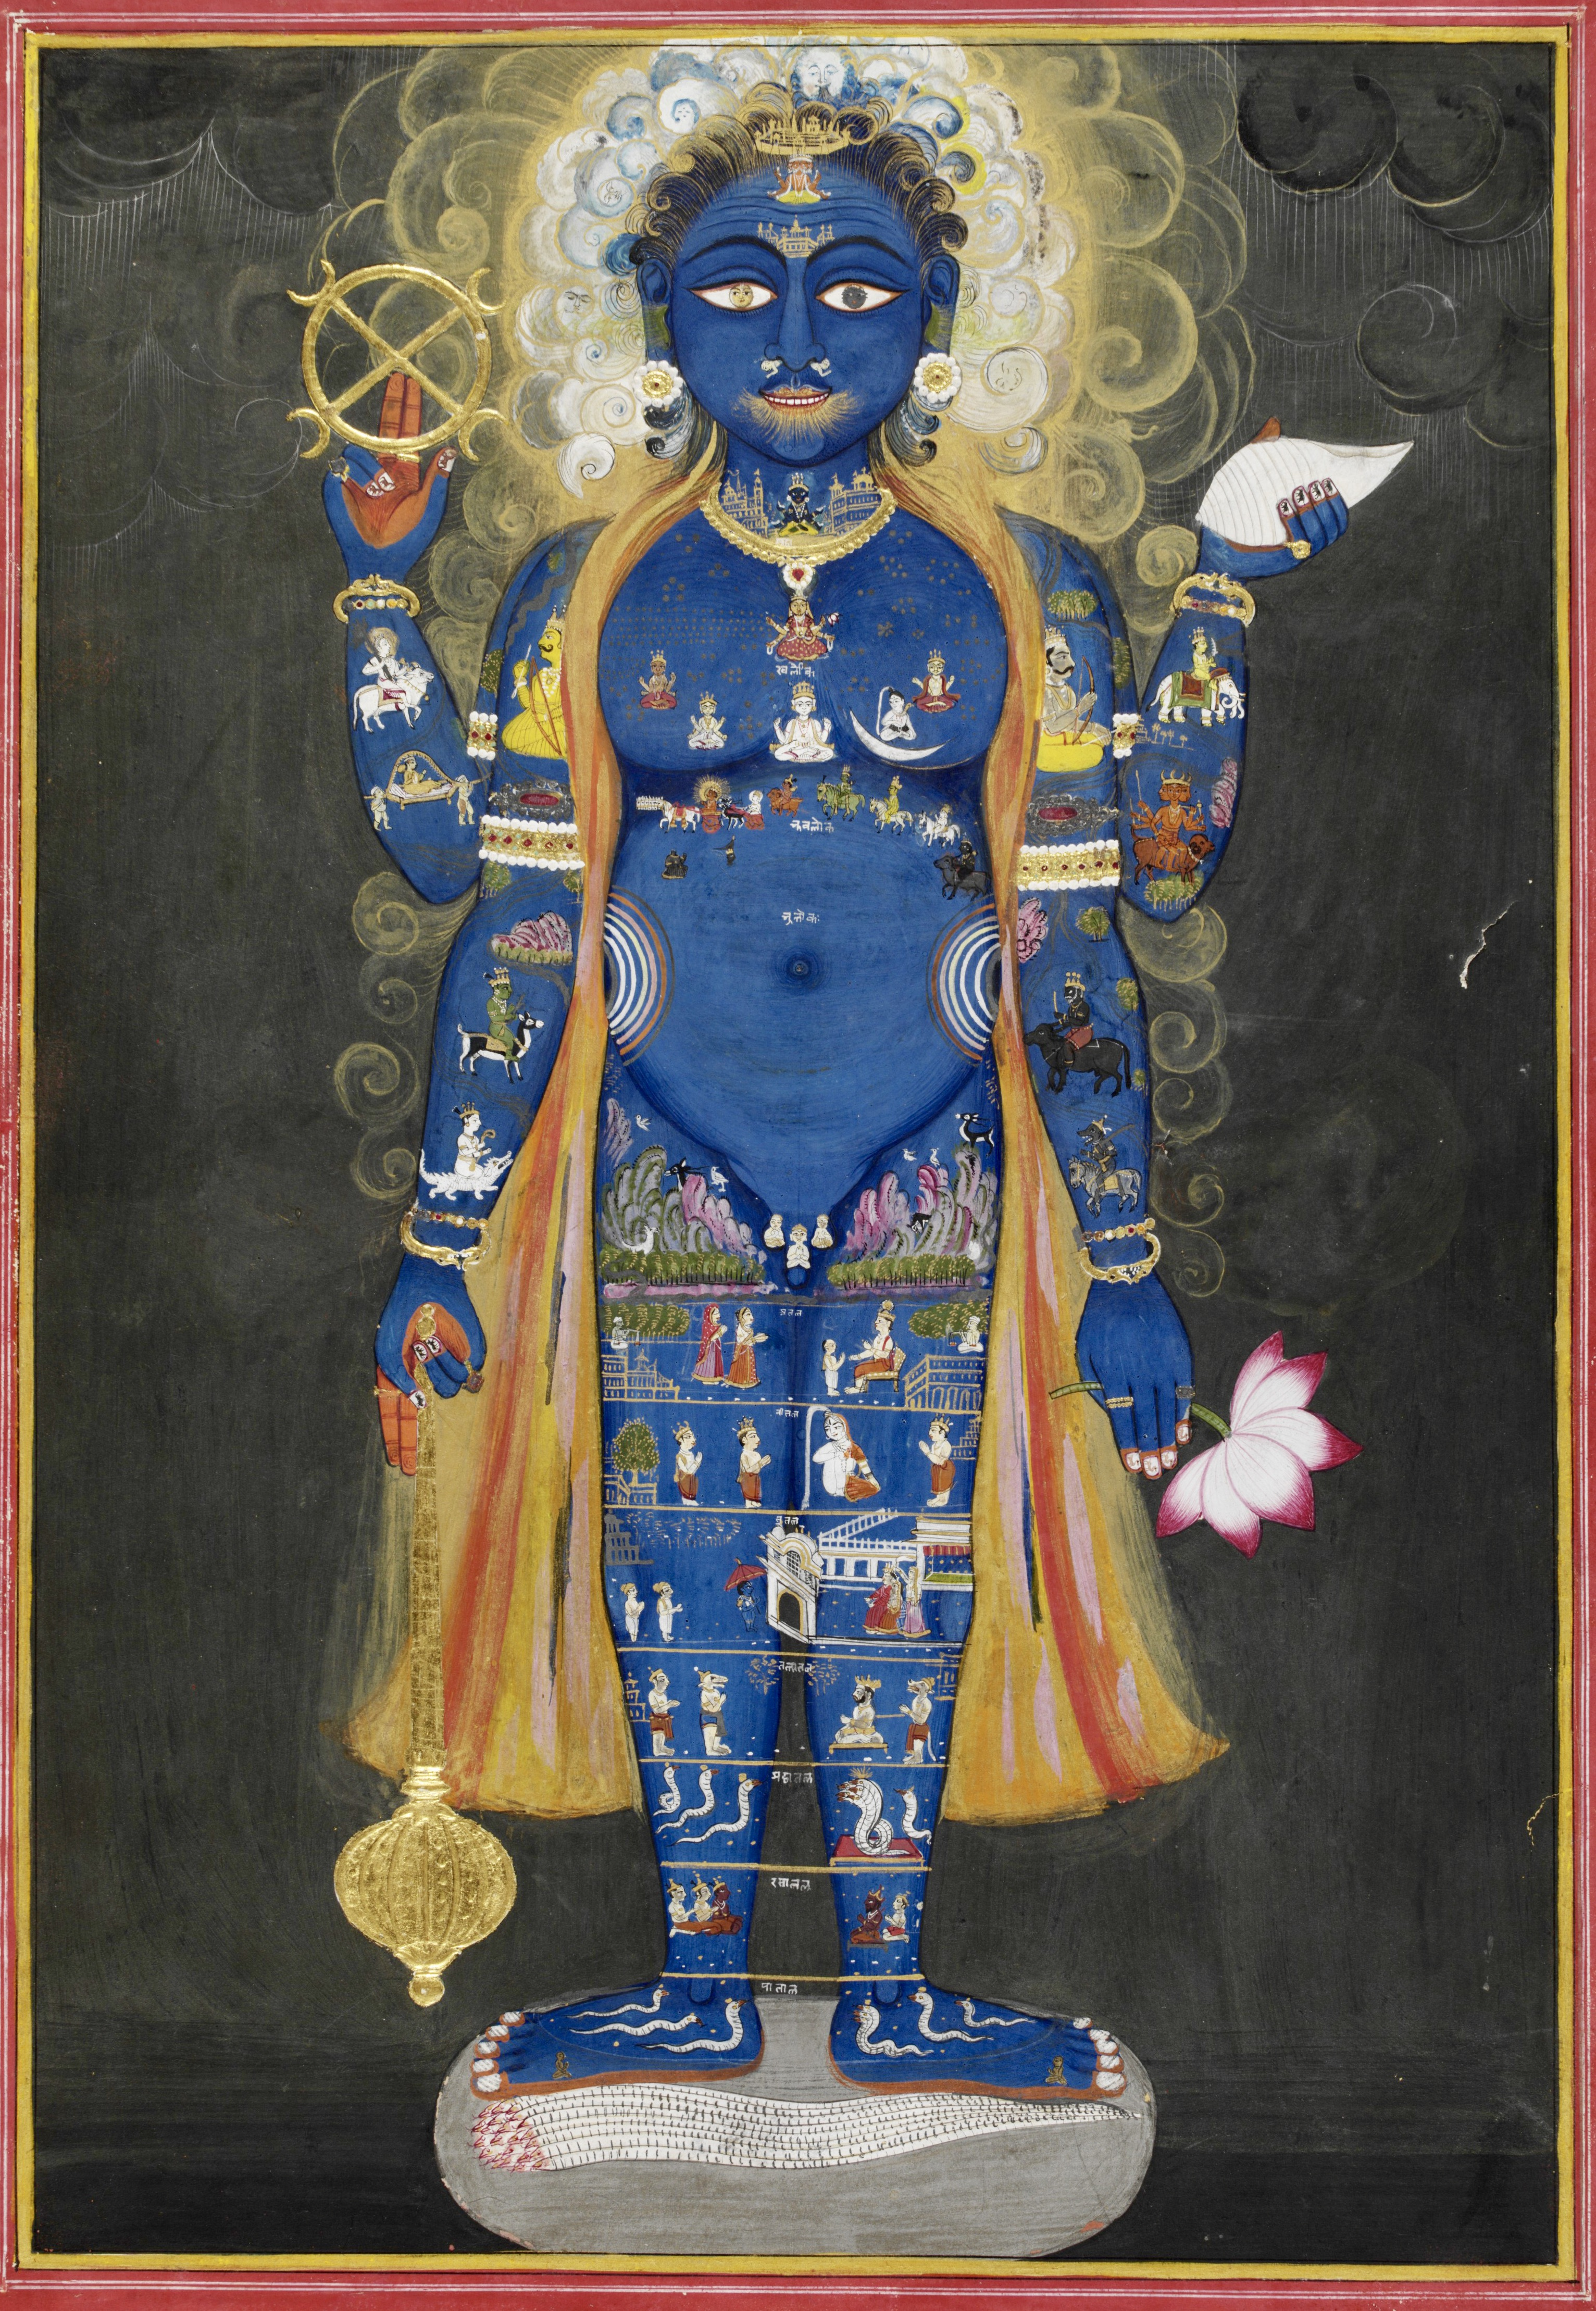
\includegraphics[width=1\textwidth]{pics/Vishnu_Vishvarupa_cropped.jpg}
	\caption{Viṣṇu Viśvarūpa, India, Rajasthan, Jaipur, ca. 1800–1820, Opaque watercolor and gold on paper, 38.5 × 28 cm, Victoria and Albert Museum, London, Given by Mrs. Gerald Clark.}
	\label{fig1}
      \end{figure}
\clearpage
  \begin{figure}[ht]
	\centering
  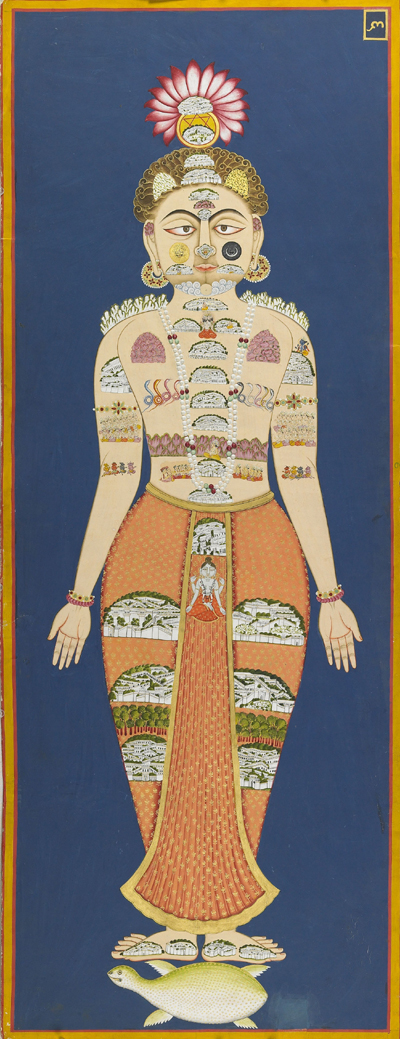
\includegraphics[width=0.5\textwidth]{pics/The_Equivalence_of_Self_and_Universe_(detail),_folio_6_from_the_Siddha_Siddhanta_Paddhati,_(Bulaki),_1824_(Samvat_1881);_122_x_46_cm._Mehrangarh_Museum_Trust..jpg}
	\caption{The Equivalence of Self and Universe (detail), folio 6 from the \textit{Siddhasiddhāntapaddhati} (Bulaki), India, Rajasthan, Jodhpur, 1824 (Samvat 1881), 122 x 46 cm, RJS 2378, Mehragarh Museum Trust.}
	\label{fig2}
      \end{figure}
      % \end{landscape}


\chapter{Bibliography}
 \label{sec:bibli}
   \clearpage
\newpage 
\thispagestyle{empty}
\quad  \addtocounter{page}{-1}

\printbibliography[heading=subbibintoc, title=Consulted Manuscripts, keyword=codex]

\printbibliography[heading=subbibintoc, title=Printed Editions, keyword=printsource]

\printbibliography[heading=subbibintoc, title=Secondary Literature, keyword=seclit]

\printbibliography[heading=subbibintoc, title=Online Sources, keyword=onlinesource]

\end{document}
